% \begin{frame}
%     \frametitle{Empirical applications: Gobi Desert}
%     \vspace{-2mm}
%     \begin{columns}
%         % \column{\dimexpr\paperwidth-10pt}
%         \column{\dimexpr\paperwidth}
%         \includegraphics[width=\textwidth]{/home/jamie/Dropbox/field-photos/gobi/mongolia-auto-shop.jpg}
%     \end{columns}
% \end{frame}

% \begin{frame}
%     \frametitle{Empirical applications: Gobi Desert}
%     \vspace{-2mm}
%     \begin{columns}
%         % \column{\dimexpr\paperwidth-10pt}
%         \column{\dimexpr\paperwidth}
%         \includegraphics[width=\textwidth]{/home/jamie/Dropbox/field-photos/gobi/mongolia-teratoscincus-przewalskii-landscape.jpg}
%     \end{columns}
% \end{frame}

\begin{frame}
    \frametitle{Empirical applications: West-Central Africa}
    \begin{columns}
        \column{0.5\linewidth}
        % \begin{minipage}[c][\textheight][c]{\columnwidth}
        \begin{itemize}
            \item Did climate cycles drive diversification and community
                assembly across rainforest taxa?
            \item<2-> Funded by NSF
            \item<3-> Preliminary results with 300 loci from 3 taxa
        \end{itemize}

        \begin{minipage}[c][0.45\textheight][c]{\columnwidth}
        \begin{center}
            \only<1-2>{
            \includegraphics[height={2.5cm}]{/home/jamie/Dropbox/field-photos/people/adam.png}
            \hspace{0.3mm}
            \includegraphics[height={2.5cm}]{/home/jamie/Dropbox/field-photos/people/fujita.jpg}
            }

            \includegraphics<3->[width=0.9\columnwidth]{../images/number-of-divs-africa.pdf}
        \end{center}
        \end{minipage}

        \column{0.5\linewidth}
        % \begin{minipage}[c][\textheight][c]{\columnwidth}
        {\centering
            \includegraphics[width=\columnwidth]{/home/jamie/Dropbox/field-photos/africa/Figure2_WAmapForestDist.png}
            
            \vspace{5mm}

            \includegraphics[width=\columnwidth]{/home/jamie/Dropbox/field-photos/africa/Figure4_herps.jpeg}

        }
        % \end{minipage}
    \end{columns}
\end{frame}

\begin{frame}
    \frametitle{Empirical applications: Gobi Desert}
    \begin{columns}
        \column{0.5\linewidth}
        % \begin{minipage}[c][\textheight][c]{\columnwidth}
        \begin{itemize}
            \item Did the formation of the Gobi cause co-diversification
                across rock and sand-adapted communities of lizards?
            \item<2-> Funding from National Geographic Society to
                survey lizard biodiversity and collect preliminary
                genetic data
        \end{itemize}

        \column{0.5\linewidth}
        % \begin{minipage}[c][\textheight][c]{\columnwidth}
        {\centering
            \includegraphics[width=\columnwidth]{/home/jamie/Dropbox/field-photos/gobi/mongolia-auto-shop.jpg}

            \vspace{2mm}
            \includegraphics[width=\columnwidth]{/home/jamie/Dropbox/field-photos/gobi/mongolia-teratoscincus-przewalskii-landscape.jpg}
        }
        % \end{minipage}
    \end{columns}
\end{frame}

\begin{frame}
    \frametitle{Empirical applications: Southeast Asia}
    \begin{columns}
        \column{0.5\linewidth}
        \begin{itemize}[<+->]
            \item Did glacial cycles promote co-diversification across SE Asia?
            \item Compare patterns of diversification between continental and
                oceanic island systems
            \item Islands of the Sunda Shelf are an exciting system for
                comparative evolutionary biology
            \item NSF pre-proposal pending
        \end{itemize}
        
        \column{0.5\linewidth}
        {\centering
            {\setlength{\fboxsep}{0pt}
            \fbox{
                \hspace{-1.2mm}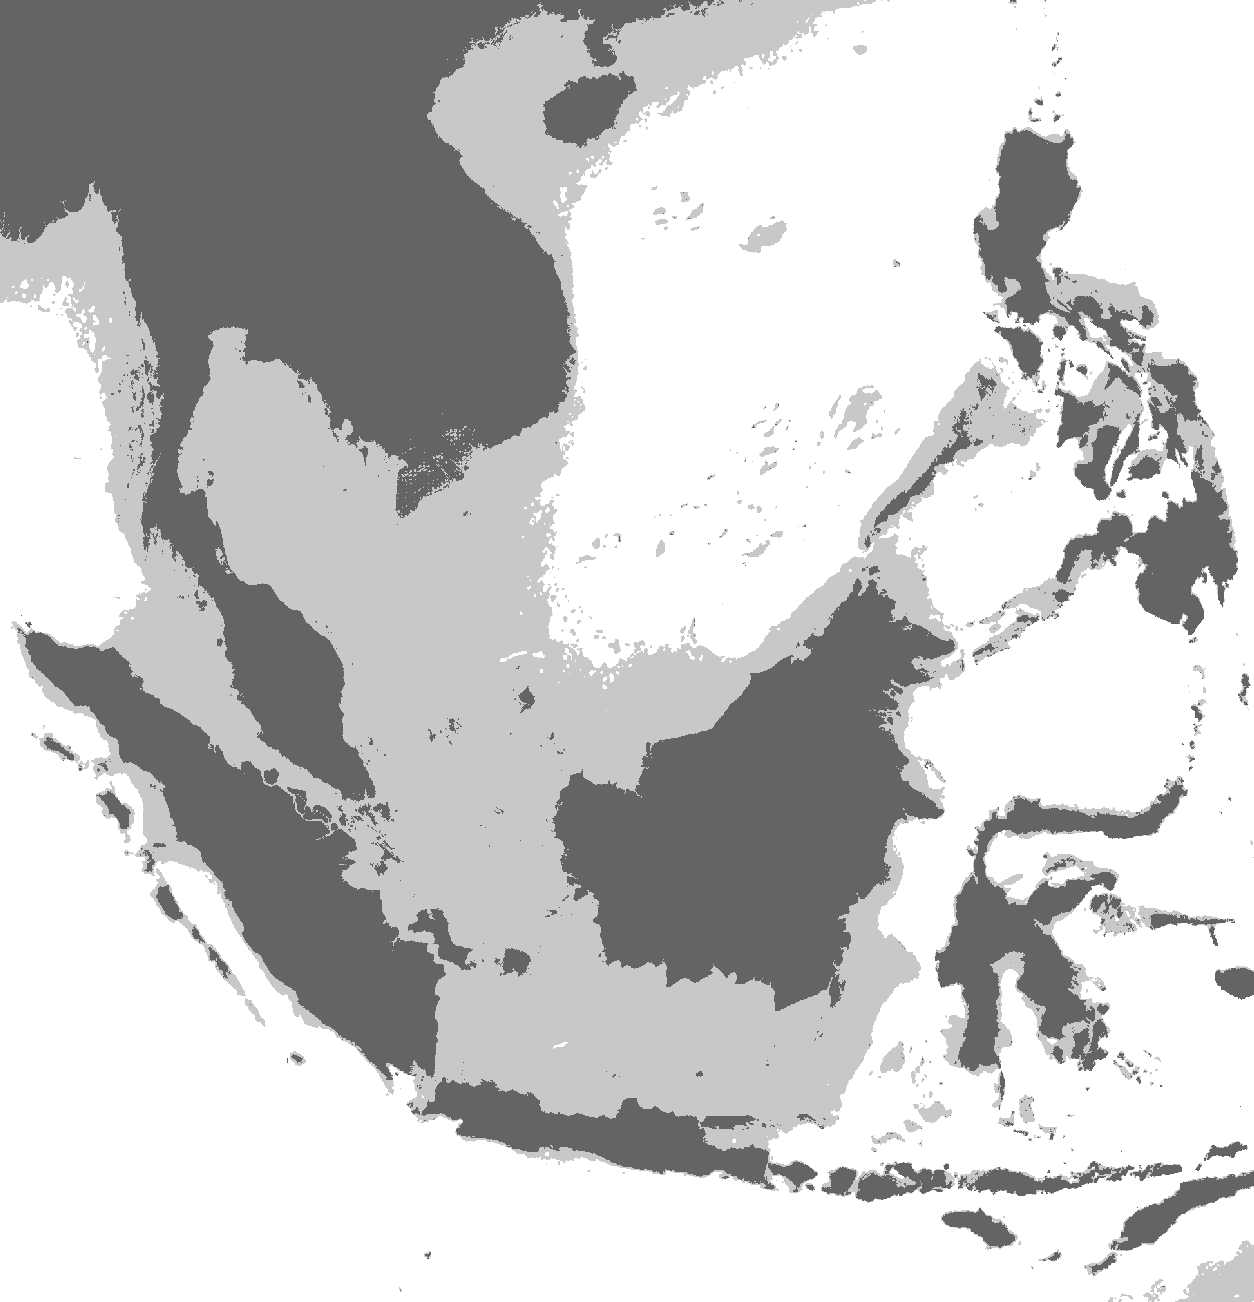
\includegraphics[width=\columnwidth]{../images/maps/se-asia-120-crop.png}
            }}
        }
    \end{columns}
\end{frame}

